%%%%%%%%%%%%%%%%%%%%%%%%%%%%%%%%%%%%%%%%%%%%%%%%%%%%%%%%%%%%%%%%%%%%%%%%%%%%%%%%
% Appendix-B.tex: Particle tracking
%%%%%%%%%%%%%%%%%%%%%%%%%%%%%%%%%%%%%%%%%%%%%%%%%%%%%%%%%%%%%%%%%%%%%%%%%%%%%%%%
% Outline:
% - Cross-correlation tracking method
% - Fourier transform based orientation analysis
%%%%%%%%%%%%%%%%%%%%%%%%%%%%%%%%%%%%%%%%%%%%%%%%%%%%%%%%%%%%%%%%%%%%%%%%%%%%%%%%
\chapter{Image Analysis implementations}

\section{Code Vectorization}
\subsection{Vectorized Code for Spatial Correlation Function}
\begin{minted}
[
frame=lines,
framesep=2mm,
baselinestretch=1.1,
linenos,
]
{python}

def corrS(X, Y, U, V):
    row, col = X.shape
    vsqrt = (U ** 2 + V ** 2) ** 0.5
    U = U - U.mean()
    V = V - V.mean()
    Ax = U / vsqrt
    Ay = V / vsqrt
    CA = np.ones(X.shape)
    CV = np.ones(X.shape)
    for xin in range(0, col):
        for yin in range(0, row):
            if xin != 0 or yin != 0:
                CA[yin, xin] = (Ax[0:row-yin, 0:col-xin] * Ax[yin:row, xin:col] + Ay[0:row-yin, 0:col-xin] * Ay[yin:row, xin:col]).mean()
                CV[yin, xin] = (U[0:row-yin, 0:col-xin] * U[yin:row, xin:col] + V[0:row-yin, 0:col-xin] * V[yin:row, xin:col]).mean() / (U.std()**2+V.std()**2)
    return CA, CV
\end{minted}

\subsection{Non-vectorized Code for Spatial Correlation Function}
\begin{minted}
[
frame=lines,
framesep=2mm,
baselinestretch=1.1,
linenos,
]
{python}
def corrS(X, Y, U, V):
    row, col = X.shape
    vsq = 0
    CA = np.zeros((row, col))
    CV = np.zeros((row, col))
    for i in range(0, row):
        for j in  range(0, col):
            vsq += U[i, j]**2 + V[i, j]**2
    for xin in range(0, col):
        for yin in range(0, row):
            count = 0
            CAt = 0
            CVt = 0
            for i in range(0, col-xin):
                for j in range(0, row-yin):
                    ua = U[j, i]
                    va = V[j, i]
                    ub = U[j+yin, i+xin]
                    vb = V[j+yin, i+xin]
                    CAt += (ua*ub+va*vb)/((ua**2+va**2)*(ub**2+vb**2))**.5
                    CVt += ua*ub + va*vb
                    count += 1
            CA[yin, xin] = CAt / count
            CV[yin, xin] = CVt / vsq
    return CA, CV
\end{minted}


\begin{figure}[!ht]
	\begin{center}
	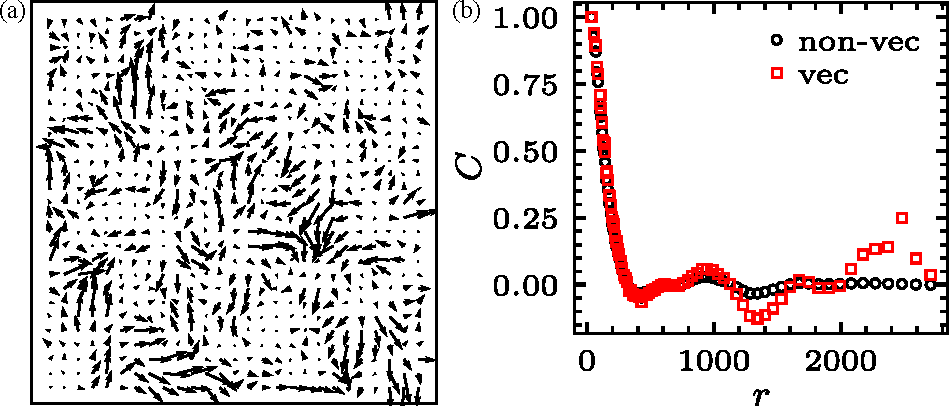
\includegraphics[width=5.5in]{Figs/A-2/vectorization.pdf}
	%select pdftexify command to run jpg or pdf files
	\end{center}
	\caption[Compare the performance of vectorized and non-vectorized code]
	{
	\textbf{Compare the performance of vectorized and non-vectorized code.}
  (a) Sample velocity field.
  (b) Velocity correlation functions obtained from the vectorized and non-vectorized code.
	}
	\label{fig:vectorization-performance}
\end{figure}


\subsection{Performance Comparison}
We notice that the vectorized code has two less nested \texttt{for} loops compared to the non-vectorized code. As a result, the vectorized one runs much faster for the same task. To quantify this performance difference, we perform the spatial correlation function calculation using both code on the same velocity field, shown in Fig.~\ref{fig:vectorization-performance}a. The times taken for the two functions are:
\begin{itemize}
  \item \texttt{Vectorized code: 0.84 s}
  \item \texttt{Vectorized code: 52.06 s}
\end{itemize}
The result is shown in Fig.~\ref{fig:vectorization-performance}b. Although in the large $r$ regime, two methods show descrepancies, in the meaningful small $r$ regime, two methods give exactly the same results.


\section{Energy Spectrum Calculation}

\section{Cross-correlation Tracking Method}
\label{cross-correlation-tracking-method}
% This is designed for tracking colloidal chains

\section{Fourier Transform Based Orientation Analysis}
\label{fourier-transform-based-orientation-analysis}

\section{Density Fluctuation Calculation}
